\subsection{DOP 11 Функции FIRST и FOLLOW. LL(l)-грамматики. Конструирование таблицы предсказывающего анализатора.}

LL(1)-анализатор -- нисходящий алгоритм синтаксического разбора. Цифра 1 говорит, что для определения пути разбора нужна всего одна лексема.

LL(1) Используется для разбора кода в ряде языков программирования, таких, как Pascal и Python (до 3.8). Очень быстр в исполнении и имеет характерное сообщение об ошибке вида «ожидался такой-то символ».

\textbf{Определения}
\begin{itemize}
    \item При построении таблицы предсказывающего анализатора нам потребуются две функции FIRST и FOLLOW.
    \item Пусть $G = (N, T, P, S)$ --- КС-грамматика. 
    Для $\alpha$ --- произвольной цепочки, состоящей из символов грамматики, --- определим FIRST($\alpha$) как множество терминалов, с которых начинаются строки, выводимые из $\alpha$. 
    Если $\alpha \Rightarrow^\ast e$, то $e$ также принадлежит FIRST ($\alpha$).
    \item Определим FOLLOW($A$) для нетерминала $A$ как множество терминалов $a$, которые могут появиться непосредственно справа от $A$ в некоторой сентенциальной форме грамматики, то есть множество терминалов $a$ таких, что существует вывод вида $S \Rightarrow^\ast \alpha A a \beta$ для некоторых $\alpha,~\beta \in (N \cup T)^\ast$.
    Заметим, что между $A$ и $a$ в процессе вывода могут находиться нетерминальные символы, из которых выводится $e$. 
    Если $A$ может быть самым правым символом некоторой сентенциальной формы, то $e$ также принадлежит FOLLOW ($A$).
    \item Грамматика $G = (N, T, P, S)$ является \textit{$LL(1)$-грамматикой} тогда и только тогда, когда для каждой пары правил $A \rightarrow \alpha$, $A \rightarrow \beta$ из P (то есть правил с одинаковой левой частью) выполняются следующие 2 условия:
    \begin{enumerate}
        \item $\text{FIRST}(\alpha) \cap \text{FIRST}(\beta) = \varnothing$.
        \item Если $e \in \text{FIRST}(\alpha)$, то $\text{FIRST}(\beta) \cap \text{FOLLOW}(A) = \varnothing$.
    \end{enumerate}
\end{itemize}

\textbf{Вычисление FIRST для символов КС грамматики}

\textit{Вход:} КС грамматика $G = (N, T, P, S)$.

\textit{Выход:} Множество FIRST($X$) для каждого символа $X \in (N \cup T)$.

\begin{enumerate}
    \item Если $X$ --- терминал, то положить $\text{FIRST}(X) = \{X\}$, если нетерминал --- $\text{FIRST}(X) = \varnothing$.
    \item Если в $P$ есть правило $X \rightarrow e$, то добавить в FIRST(X) $e$.
    \item Выполнять алгоритм на рисунке ниже.
    
    Краткое описание: для каждого правила $X \leftarrow Y_1 Y_2 \dots$ в FIRST($X$) добавлять FIRST($Y_1$) и, если $e \in \text{FIRST}(Y_1)$, добавлять FIRST($Y_2$) и, если $e \in \dots$. 
\end{enumerate}

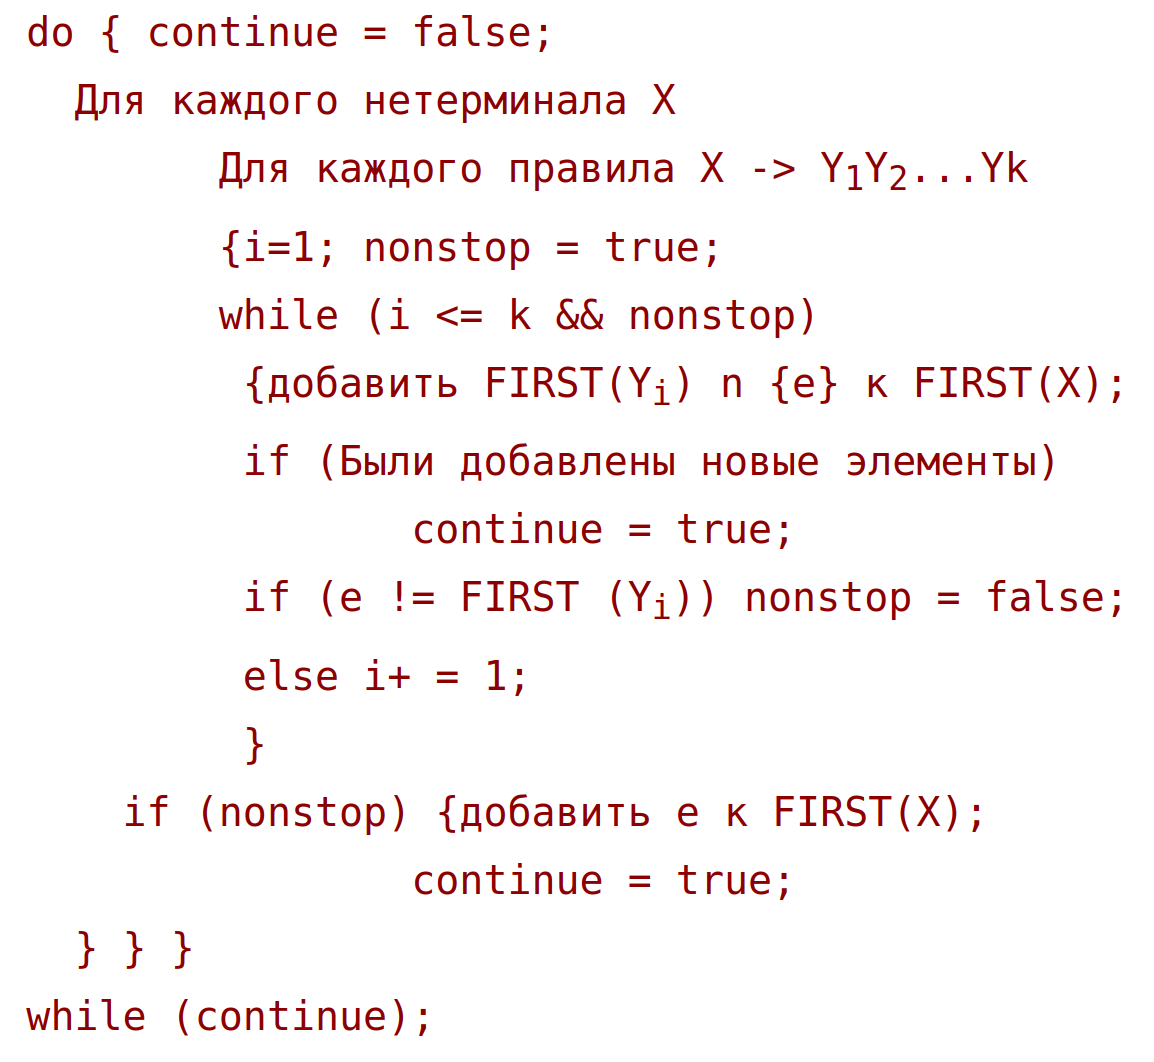
\includegraphics[width=0.2\textwidth]{pics/first.png}

\textbf{Вычисление FIRST для цепочки}

\textit{Вход:} КС грамматика $G = (N, T, P, S)$.

\textit{Выход:} Множество FIRST($X_1, X_2, \dots, X_n$), $X_i \in (N \cup T)$.


\begin{enumerate}
    \item Для всех $X \in (N \cup T)$ вычислить FIRST($X$).
    \item Положить FIRST($X_1, X_2, \dots, X_n$) $ = \varnothing$.
    \item Выполнить алгоритм на рисунке ниже \newline
    Краткое описание: добавляем во множество FIRST($X_1$), и, если $e \in \text{FIRST}(X_1)$, FIRST($X_2$), и, если $e \in \dots$.
\end{enumerate}

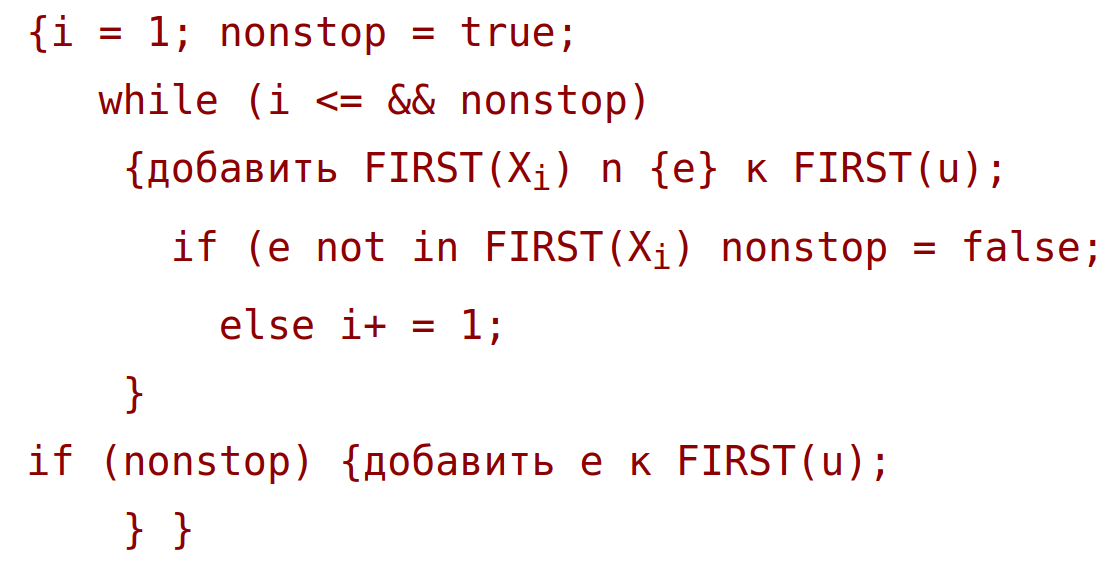
\includegraphics[width=0.2\textwidth]{pics/firstc.png}

\textbf{Вычисление FOLLOW для нетерминалов грамматики}

\textit{Вход:} КС грамматика $G = (N, T, P, S)$.

\textit{Выход:} Множество FOLLOW($X$) для каждого символа $X \in N$.

\begin{enumerate}
    \item FOLLOW($X$) $= \varnothing$ для каждого знака $X \in N$.
    \item Добавить \$ к FOLLOW($S$).
    \item Если в $P$ есть правило вывода $A \rightarrow \alpha B \beta, \alpha,~\beta \in (N \cup T)^\ast$, то все элементы из FIRST($\beta$), кроме $e$, добавляем к FOLLOW($B$).
    \item если в $P$ есть правило $A \rightarrow \alpha B$ или $A \rightarrow \alpha B \beta,~\alpha,~\beta \in (N \cup T)^\ast$, где FIRST($\beta$) содержит $e$, то есть $\beta \Rightarrow^\ast = e$, то все элементы из FOLLOW ($A$) добавить к FOLLOW ($B$).
    \item Продолжать шаги 2 и 3, пока какие-то множества меняются.
\end{enumerate}

\textbf{Конструирование таблицы предсказывающего анализатора по грамматике $G$}.
Пусть $A \rightarrow \alpha$ --- правило вывода грамматики и $a \in \text{FIRST}(\alpha)$. 
Тогда анализатор делает развертку $A$ по $\alpha$, если входным символом является $a$. 
Трудность возникает, когда $\alpha = e$ или $\alpha \Rightarrow e$. 
В этом случае нужно развернуть $A$ в $\alpha$, если текущий входной символ принадлежит FOLLOW($A$) или если достигнут \$ и $\$ \in \text{FOLLOW}(A)$.

\textit{Алгоритм}

\textit{Вход:} КС-грамматика $G = (N, T, P, S)$.

\textit{Выход:} Таблица $M[A, a]$ предсказывающего анализатора, $A \in N,~a \in T \cup \{\$\}$.

Для каждого правила вывода $A \rightarrow \alpha$ грамматики выполнить шаги 1 и 2. После этого выполнить шаг 3.
\begin{enumerate}
    \item Для каждого терминала $a$ из FIRST($\alpha$) добавить $A \rightarrow \alpha$ к $M[A, a]$.
    \item Если $e \in \text{FIRST}(\alpha)$, добавить $A \rightarrow \alpha$ к $M[A, b]$ для каждого терминала $b$ из FOLLOW ($A$).
    Кроме того, если $e \in \text{FIRST}(\alpha)$ и $\$ \in \text{FOLLOW}(A)$, добавить $A \rightarrow \alpha$ к $M[A, \$]$.
    \item Положить все неопределенные входы равными <ошибка>. 
\end{enumerate}

Алгоритм построения таблиц может иметь более одного правила в одной клетке
\begin{enumerate}
\item Неоднозначные грамматики
\item Леворекурсивные грамматики
\end{enumerate}

Построена таблица, в которой каждая строка соотносится с некоторым состоянием, каждый столбез -- с терминалом, а в ячейках содержатся формулы преобразований. Данная таблица используется для определения следующего состояния.

Грамматики, для которых таблица предсказывающего анализатора не имеет неоднозначно определённых ячеек, называются LL(1)-грамматика:
\begin{enumerate}
\item Сканирование слева-направо
\item Левое порождение
\item Предпросмотр 1 символа
\end{enumerate}

Язык называют LL(1)-языком, если для него существует LL(1)-грамматика \newline
Для произвольной LL(1)-грамматики G алгоритм строит таблицу
предсказывающего анализатора, распознающего все цепочки из L(G) и только их.\newline
Если G — LL(1)-грамматика, то L(G) — детерминированный КС-язык.


% -------- source --------
\bigbreak
[\cite[page 69-96]{replace_me}]